% 3

\chapter{Analisi e progettazione}

% 3.1

\section{Descrizione del problema}

Si vuole realizzare un'applicazione desktop per l'analisi di bilancio di un'azienda per l'ordine dei commercialisti della provincia di Ancona.
L'applicazione sarà resa scaricabile dal sito dell'Ordine e deve essere operativa per i vari tipi di sistema operativo, perciò il software deve essere cross-platform.
Per poter realizzare un prodotto che sia cross-platform, ossia implementato per più piattaforme di elaborazione, la scelta delle tecnologie da utilizzare è stata fondamentale.
Quando si vuole sviluppare un'applicazione desktop la prima cosa a cui si pensa è per quale sistema operativo svilupparla, quale linguaggio usare ed opzionalmente a quale base dati si ha bisogno di connettersi.
Il mondo dell'informatica intanto si sta evolvendo verso l'utilizzo di applicazioni web per la loro semplicità di distribuzione e aggiornamento, la compatibilità con ogni sistema operativo e la superfluità di un'installazione, allora perchè non sfruttare questa tecnologia?
Per questo la scelta è ricaduta su un compromesso valido, Electron.
Definita dallo slogan "Build cross platform desktop apps with Javascript, HTML, and CSS", Electron è una libreria open source sviluppata dal team di GitHub che permette di sviluppare un’applicazione desktop utilizzando le stesse tecnologie di un sito web, unendo la potenza del browser Chromium, la flessibilità di Node.js e il più grande ecosistema di librerie open source al mondo: npm. In aggiunta a tutto questo la possibilità di pacchettizzare l’applicazione per Mac, Windows, e Linux con lo stesso risultato in termini di grafica e funzionalità.

L'applicazione realizzata, nello specifico, dovrà permettere all'utente che la utilizza l'inserimento in input dei dati relativi all'Anagrafica, all'Analisi Qualitativa, dello Stato Patrimoniale e del Conto Economico.
Nella fase di inserimento dei valori dello Stato Patrimoniale e del Conto Economico, il sistema calcola tramite formule pre-impostate, le varie riclassificazioni dello Stato Patrimoniale (Funzionale, Finanziario o entrambi) e del Conto Economico (al Valore Aggiunto).
L'utente deve avere la possibilità di salvare in corso d'opera il progetto e poterlo riaprire in un secondo momento.
Inoltre, va implementata una funzione che permette la stampa in un file pdf del progetto.


% 3.2

\section{Analisi dei requisiti}

Al fine di esporre i requisiti in maniera rigorosa, verrà adottata la notazione MoSCoW, la quale fa uso delle seguenti etichette:
\begin{itemize}
\item Must Have: sottolinea un requisito di fondamentale importanza per il funzionamento del sistema;
\item Should Have: indica un requisito importante ma non essenziale per il funzionamento del sistema;
\item Could Have (o Nice to Have): indica un requisito non importante come i precedenti e volto principalmente a migliorare la soddisfazione del cliente.
\item Won’t Have: requisiti che non devono essere implementati (negazione di una funzione).
\end{itemize}

% 3.2.1

\newpage

\subsection{Requisiti funzionali}
I requisiti funzionali descrivono le funzionalità del sistema software, in termini di servizi che il sistema software deve fornire, di come il sistema software reagisce a specifici tipi di input e di come si comporta in situazioni particolari.

\begin{table}[H]
    \footnotesize
    \centering
    \begin{tabulary}{0.9\textwidth}{|L|L|c|}
        \hline
        ID & Descrizione & MoSCoW \\
        \hline\hline
        1 & Il programma deve permettere l'inserimento e la visualizzazione dei dati di un'azienda del progetto & Must have \\
        \hline
        2 & Il programma deve permettere il salvataggio del progetto & Must have \\
        \hline
        3 & Il programma deve permettere la lettura di un progetto salvato in precedenza & Must have \\
        \hline
        4 & Il programma deve permettere la stampa in un formato pdf del progetto & Must have \\
        \hline
        5 & Il programma dovrebbe permettere di inserire solamente valori numerici per i campi in cui vengono inseriti le valute & Should have \\
        \hline
        10 & Il programma potrebbe permettere il download in un formato open-data (CSV) delle fatture trovate & Could have \\
        \hline
        11 & Il programma non deve permettere di creare mandati e decreti che non siano già presenti negli altri gestionali specifici & Won't have \\
        \hline
    \end{tabulary}
    \caption{Requisiti funzionali}
\end{table}

% 3.2.2

\newpage

\subsection{Requisiti non funzionali}
Descrivono le proprietà del sistema software in relazione a determinati servizi o funzioni e possono anche essere relativi al processo:
\begin{itemize}
\item Caratteristiche di efficienza, affidabilità, safety, ecc.
\item Caratteristiche del processo di sviluppo (standard di processo, linguaggi di programmazione, metodi di sviluppo, ecc.
\item Caratteristiche esterne (interoperabilità con sistemi di altre organizzazioni, vincoli legislativi, ecc.)
\end{itemize}

\begin{table}[H]
    \footnotesize
    \centering
    \begin{tabulary}{0.9\textwidth}{|L|L|c|}
        \hline
        ID & Descrizione & MoSCoW \\
        \hline\hline
        1 & Il programma deve essere sviluppato per tutte le piattaforme di elaborazione & Must have \\
        \hline
        2 & Il programma deve essere interoperabile con il software del protocollo (Paleo) per quanto riguarda la ricezione di messaggi di assegnazione RP alle fatture & Must have \\
        \hline
        3 & Il programma deve essere interoperabile con il software dei decreti (OpenAct) per la ricezione dei decreti di pagamento fatture & Must have \\
        \hline
        4 & Il programma deve essere interoperabile con il software della contabilità (Siagi) per la ricezione dei mandati di pagamento e l'invio delle informazioni sulle fatture per la comunicazione alla \Gls{pcc} & Must have \\
        \hline
        5 & Deve essere garantita la consistenza tra le informazioni presenti nel programma e quelle presenti negli altri programmi gestionali collegati & Must have \\
        \hline
        6 & Il sito dovrebbe essere visibile da ogni browser (cross-browser) & Should have \\
        \hline
        7 & La navigazione del sito, in particolar modo il caricamento delle pagine di ricerca, dovrebbe essere veloce & Should have \\
        \hline
        8 & Il sito può essere adattabile alle differenti risoluzioni dello schermo (responsive) & Could have \\
        \hline
    \end{tabulary}
    \caption{Requisiti non funzionali}
\end{table}

% 3.2.3

\newpage

\subsection{Requisiti di dominio}
Si tratta di requisiti derivati dal dominio applicativo del sistema software piuttosto che da necessità dettate dagli utenti. Sono pertanto requisiti del tutto ovvi a persone che lavorano nel dominio (vedi esistenza di leggi giuridiche, regola matematica, legge fisica, ecc.) e sono spesso difficili da capire per chi non ha conoscenze nel dominio stesso.

\begin{table}[H]
    \footnotesize
    \centering
    \begin{tabulary}{0.9\textwidth}{|L|L|c|}
        \hline
        ID & Descrizione & MoSCoW \\
        \hline\hline
        1 & Il database del programma deve essere in un server \Gls{mssql} & Must have \\
        \hline
        2 & Il sito deve essere ospitato da una macchina Windows Server 2008 o superiore con \Gls{iis} e \Gls{net} installati & Must have \\
        \hline
        3 & Il programma deve rispettare gli obblighi previsti dalla normativa italiana in materia di fatturazione elettronica & Must have \\
        \hline
        4 & Il programma deve essere in grado di interpretare i dati della fattura xml inviata da \Gls{imm} e definiti nelle regole tecniche dell'Agenzia delle Entrate & Must have \\
        \hline
        5 & Il sito deve soddisfare i criteri di accessibilità e usabilità descritti nella legge Stanca della normativa italiana sui siti web della \Gls{pa} & Must have \\
        \hline
    \end{tabulary}
    \caption{Requisiti di dominio}
\end{table}

% 3.3

\newpage

\section{Use case diagram}

Gli Use Case Diagrams descrivono il comportamento funzionale del sistema, come visto dall’utente. Sono diagrammi di facile interpretazione dove abbiamo uno o più attori che possono attivare diverse funzioni/servizi all'interno di uno o più sistemi.

\begin{figure}[H]
    \centering
    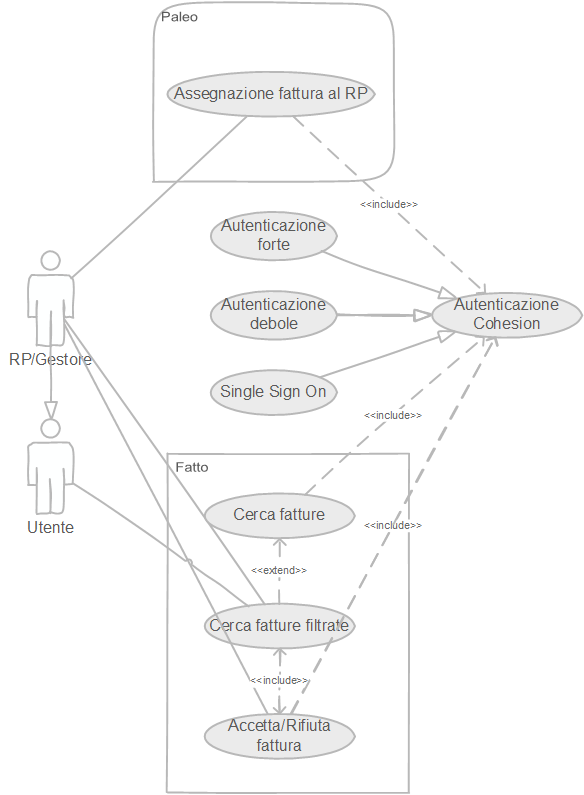
\includegraphics[scale=0.7]{use-case-diagram-v2.png}
    \caption{UML Use Case Diagram - accettazione}
    \label{fig:UseCase1}
\end{figure}

Nel diagramma in figura  ~\ref{fig:UseCase1} abbiamo due attori, RP/Gestore e Utente, il secondo è la generalizzazione del primo, questo significa che tutti i casi d'uso che valgono per il secondo valgono anche per il primo, ma non viceversa.
I casi d'uso talvolta includono più passaggi al loro interno, in quei casi è indacata una freccia "include", come nel caso della "Ricerca fatture" che include "Autenticazione Cohesion".
Alcuni casi d'uso sono estensione di altri, in altre parole sono una "specializzazione", un esempio è la "Ricerca fatture filtrata" che è una specializzazione della "Ricerca fatture".
I riquadri indicano i diversi sistemi software e distinguono a quale di essi appartengono i vari casi d'uso.

% 3.4

\newpage

\section{Activity diagram}

L'Activity Diagram è un diagramma che definisce le attività da svolgere per realizzare una data funzionalità ed è spesso utilizzato come modello complementare dello Use Case Diagram.

\begin{figure}[H]
    \centering
    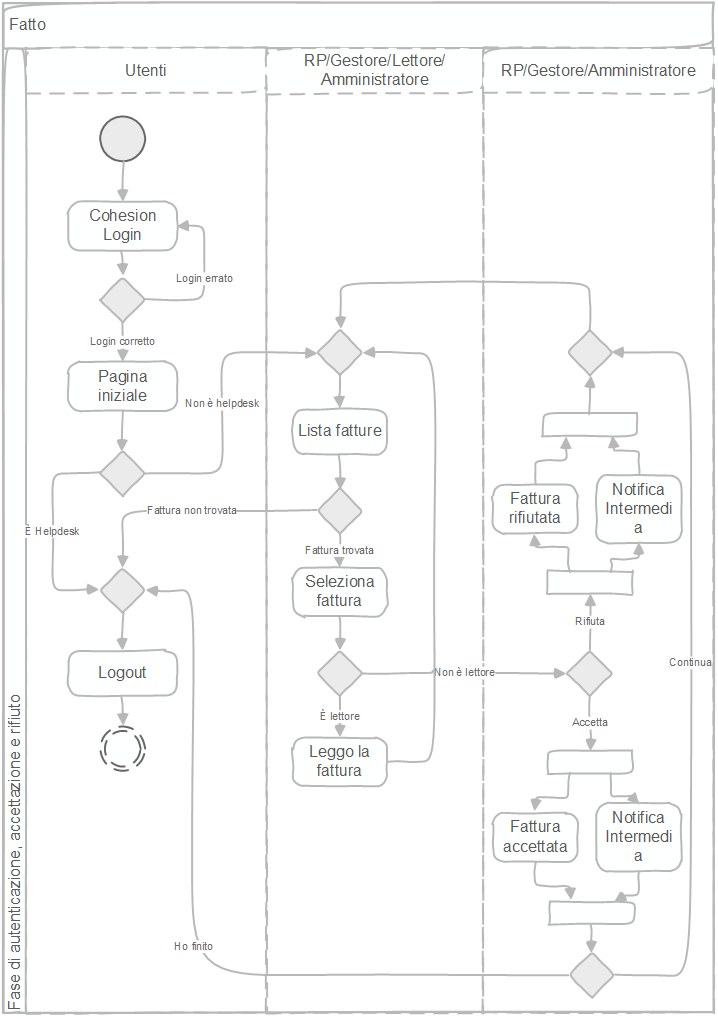
\includegraphics[scale=0.6]{activity-diagram-v2.png}
    \caption{UML Activity Diagram - autenticazione e accettazione}
    \label{fig:ActivityDiagram1}
\end{figure}

Nella figura ~\ref{fig:ActivityDiagram1} vediamo descritta la stessa fase dello Use Case precedente, cioè quella di autenticazione e accettazione/rifiuto, ma dal punto di vista delle attività da svolgere in sequenza per raggiungere un certo risultato (l'accettazione in questo caso).
Il diagramma si legge a partire dal pallino in alto, detto nodo iniziale, seguono le azioni indicate dai rettangoli verdi.
I rombi indicano le decisioni, cioè le diverse direzioni che può prendere il flusso a seguito di certe condizioni o scelte, ad esempio dopo l'azione "Cohesion login", se il login è errato si ritorna alla pagina di login, altrimenti si raggiunge la pagina iniziale.
Altri elementi dell'activity diagram sono il "fork" e la "join", dove il primo sta ad indicare che diverse azioni possono essere eseguite in parallelo, mentre la seconda indica che per passare all'azione successiva devono essere completate tutte le azioni in ingresso.
Nell'esempio il blocco che inizia con la fork e finisce con la join indica che ci sono due azioni: il salvataggio del nuovo stato accettata/rifiutata e l'invio della notifica a Intermedia; entrambe le azioni devono essere completate per proseguire, ma non importa in che ordine vengano eseguite.

% 3.5

\newpage

\section{Sequence diagram}

Il sequence diagram è uno strumento di modellazione visuale che mette in evidenza come i vari componenti di un sistema interagiscono tra di loro in relazione al tempo.

\begin{figure}[H]
    \centering
    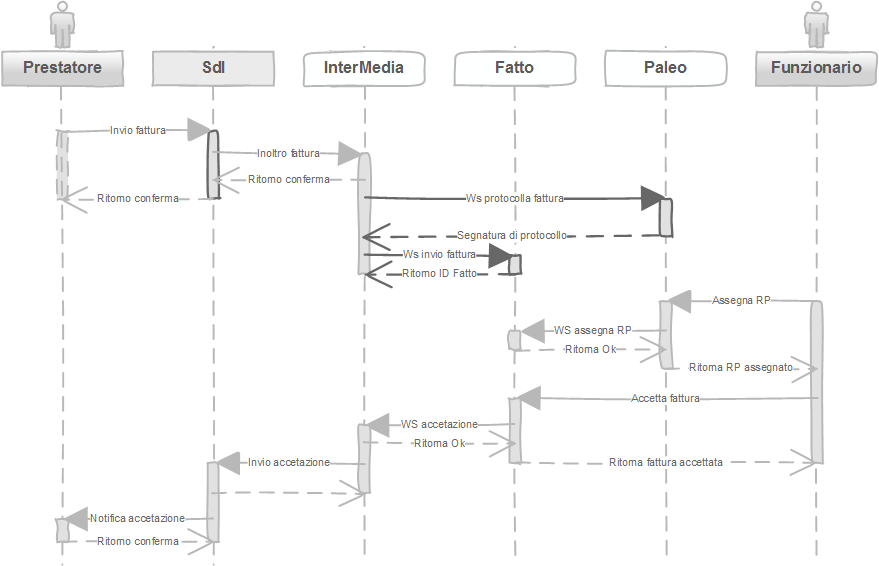
\includegraphics[scale=0.6]{sequence-diagram-v2.png}
    \caption{UML Sequence Diagram - ricezione e accettazione}
    \label{fig:SequenceDiagram}
\end{figure}

Nella figura ~\ref{fig:SequenceDiagram} vediamo descritto il flusso iniziale della fatturazione passiva che inizia con l'invio della fattura da parte del prestatore e termina con la ricezione di accettazione (in questo caso) della stessa da parte del prestatore.
I componenti del diagramma sono il prestatore, il funzionario/committente e i vari sistemi software in comunicazione tra loro tramite \Gls{ws}.
Possiamo vedere lo schema come l'unione di due operazioni:
\begin{enumerate}
\item La ricezione
\item L'accettazione
\end{enumerate}
Nella fase di ricezione il prestatore invia la fattura allo SdI, questo effettua i controlli formali e la inoltra senza modifiche al nodo di interscambio \Gls{imm}, il quale effettua un controllo della firma e spacchetta il file in caso di lotto poi invia la singola fattura, prima al  protocollo, che restituisce la segnatura (codice univoco del protocollo), poi a Fatto (il sistema di fatturazione) insieme alla segnatura.
Quando \Gls{imm} riceve la fattura ritorna allo SdI un messaggio di avvenuta ricezione il quale viene a sua volta inoltrato al prestatore.
Nella seconda fase il committente assegna un \Gls{rp} alla fattura tramite Paleo, questo comporta l'assegnazione del \Gls{rp} anche in Fatto, poi il RP in questione effettua l'accettazione da Fatto che a sua volta richiama \Gls{imm}.
Se tutto va bene \Gls{imm} risponde a Fatto che solo allora aggiorna lo stato della fattura ad "Accettata" e risponde al committente.
Infine \Gls{imm} richiama lo SdI che a sua volta avverte il prestatore dell'avvenuta accettazione.

% 3.6

\newpage

\section{Modello Entità-Relazione (E-R)}

Il modello Entità-Relazione è un modello concettuale di dati e, come tale, fornisce una serie di costrutti atti a descrivere la realtà di interesse in una maniera facile da comprendere e che prescinde dai criteri di organizzazione dei dati nei calcolatori \cite{basidati}. Tali costrutti vengono utilizzati per definire schemi che descrivono l'organizzazione e la struttura delle istanze.
I costrutti principali del modello concettuale sono:
\begin{itemize}
    \item Entità, rappresentano classi di oggetti che hanno proprietà comuni ed esistenza "autonoma" ai fini dell’applicazione di interesse. Una occorrenza di un'entità è un oggetto della classe che l'entità stessa rappresenta. In uno schema, ogni entità ha un nome che la identifica univocamente, e viene rap-presentata graficamente tramite un rettangolo con il nome dell'entità al suo interno.
    \item Relazioni (o associazioni), rappresentano legami logici, significativi per l'applicazione di interesse, tra due o più entità. Una occorrenza di relazione è un'ennupla (coppia nel caso più frequente di relazione binaria) costituita da occorrenze di entità, una per ciascuna delle entità coinvolte. Di norma viene rappresentata graficamente da un rombo contenente il nome dell'associazione. Il nome può essere un verbo in modo da fornire una direzione di lettura, oppure può essere un sostantivo in modo da non dare una direzione di lettura.
    \item Attributi, descrivono le proprietà elementari di entità o relazioni che sono di interesse ai fini dell'applicazione. Un attributo associa a ciascuna occorrenza di entità (o di relazione) un valore appartenente a un insieme detto dominio, che contiene i valori ammissibili per l’attributo. Può risultare comodo, a volte, raggruppare attributi di una medesima entità o relazione che presentano affinità nel loro significato o uso: l’insieme di attributi che si ottiene in questa maniera viene detto attributo composto.
\end{itemize}

\begin{figure}[H]
    \centering
    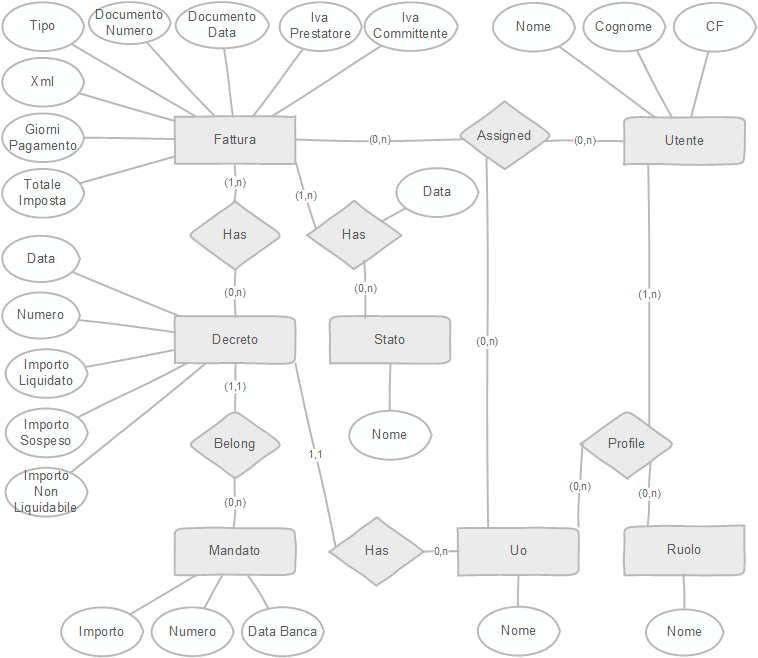
\includegraphics[scale=0.7]{er-diagram-v2.png}
    \caption{E/R Diagram}
    \label{fig:ErDiagram}
\end{figure}

Nella Figura ~\ref{fig:ErDiagram} possiamo distinguere le entità individuate da rettangoli, le relazioni rappresentate come rombi e gli attributi indicati come cerchi collegati alle entità o talvolta alle relazioni.
L'entità "Fattura" ha un attributo chiamato "Xml" che contiene il tracciato serializzato della fattura \Gls{xml}.
Una Fattura può avere zero o più Decreti, mentre un Decreto può avere una o più Fatture (non zero), un discorso simile vale per i Mandati.
Una Fattura può avere uno o più Stati, uno dei quali è sicuramente "Ricevuta"; la relazione in questo caso possiede un attributo "Data" perché gli stati sono incrementali: per vedere qual'è lo stato attuale di una Fattura si guarda semplicemente quello con la Data maggiore.
Una relazione chiamata "Assigned" collega la Fattura con l'Utente e l'UO, questa assegnazione viene fatta da Paleo tramite il \Gls{ws} di assegnazione RP.
Infine una relazione chiamata "Profile" indica l'esistenza di un profilo Ruolo-Uo per un certo Utente.